\subsubsection{Second article}
Next, we continue with the article \textit{"Learning Semantic Representations for Unsupervised Domain Adaptation"} written by Xie, Shaoan, et al. \cite{xie2018learning} The main purpose of the article is to propose a new method for unsupervised domain adaptation that utilizes semantic information to learn domain-invariant representations. The authors propose a domain adaptation algorithm which is based on the idea of using an adversarial learning to learn a feature representation that is invariant to domain shifts. 

\begin{figure}[H]
    \centering
    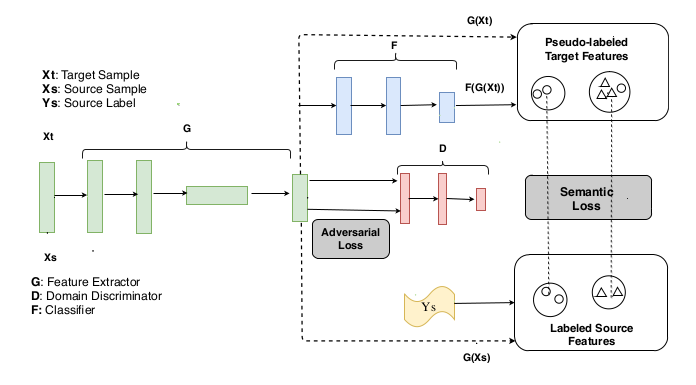
\includegraphics[width=0.7\textwidth]{Figures/From articles/sem_rep.png}
    \caption{The authors use standard source classification loss with the domain adversarial loss to align distribution for two domains. It is showed that the performance of the domain adaptation method improved significantly on several benchmark datasets by aligning the centroids. Global centroids $C_S^k$ and $C_T^k$ is maintained for each class at feature level.}
    \label{fig: sem_rep}
\end{figure}

 The authors train a feature extractor and then use it to map the input data to a high-dimensional feature space, and a domain classifier that predicts the domain label of the input data (see Figure \ref{fig: sem_rep}). The feature extractor \textbf{G} is trained to confuse the domain classifier \textbf{D}, while the domain classifier is trained to correctly predict the domain label. In this way, the feature extractor is encouraged to learn features that are invariant to domain shifts, while still being discriminative for the task.\\

 
 First, the authors denote the cross entropy loss for the source domain as $L_C(X_S, Y_S)$. Then, the discrepancy between source domain and target domain is supposed to be 

 $$
 L_{DC}(X_S, X_T) = d(X_S, X_T) = \mathbb{E}_{x \sim D_S} [\log(1 - D \circ G(x))] + \mathbb{E}_{x \sim D_T} [\log(D \circ G(x))] 
 $$
Moreover, the authors introduce one more loss, which targets the semantic representation. Centroid alignment is used for this purpose. By computing the centroid for each class, both correct and incorrect pseudo-labeled samples are utilized together: 

$$
L_{SM}(X_S, Y_S, X_T) = \sum_{k=1}^K \Phi(C_S^k, C_T^k)
$$
where $C_S^k, C_T^k$ are centroids for each class and $\Phi(x, x') = \| x - x' \|^2$. This approach aims to cancel out the negative effects caused by inaccurate pseudo labels with accurate ones. Thus, the authors get the following total loss

 $$
 L(X_S, Y_S, X_T) = L_C(X_S, Y_S) + \lambda L_{DC}(X_S, X_T) + \gamma L_{SM}(X_S, Y_S, X_T)
 $$
 where $\lambda$ and $\gamma$ are responsible for the balance between the classification
loss, domain confusion loss and semantic loss. In the article, algorithm of \textbf{moving average centroid alignment} is presented that allows to align the centroids in same class
but different domains to achieve semantic transfer for UDA.